\documentclass[adobefonts]{ctexart}
%\documentclass[winfonts]{ctexart}

\CTEXoptions[captiondelimiter={\quad}]


\usepackage{amsmath}            % AMS的数学宏包
\usepackage{amssymb}            % AMS的数学符号宏包
\usepackage{graphicx}           % 插入图片需要的宏包
\usepackage{float}              % 强大的浮动环境控制宏包
\usepackage{framed}             % `shaded'环境需要用到
\usepackage{enumitem}           % 增强列表功能
\usepackage{alltt}              % 在`alltt'环境中为等宽字体, 但可以使用LaTeX命令

% \usepackage{shortvrb}           % 简化\verb的写法
% \MakeShortVerb{\|}
\usepackage{listings}
\lstset{language=bash}
\lstset{extendedchars=false}
\lstset{breaklines}
\lstset{stepnumber=2}
\lstset{backgroundcolor=\color{lightgray}}


\usepackage{color}              % 可以定义各种颜色
\usepackage[x11names]{xcolor}   % 下面的RoyalBlue3颜色需要用到的宏包



% 自定义的几种颜色
\definecolor{shadecolor}{gray}{0.85}

% \definecolor{darkblue}{rgb}{52,101,164}
% \definecolor{darkgreen}{rgb}{78,154,6}

% % 设置背景颜色
% \definecolor{bisque}{rgb}{.996,.891,.755}
% \pagecolor{bisque}

\usepackage[pdfauthor={Dreamseeker},
  colorlinks=true,
  urlcolor=blue,
  linkcolor=RoyalBlue3]{hyperref} % 为超链接设置颜色, 修改PDF文件信息

%\CTEXsetup[name={实验,},number={\chinese{section}}]{section}


\title{\textbf{一些有用的emacs配置}}
\author{deanraccoon@gmail.com}
% \date{}

\usepackage[pagestyles]{titlesec} % 定制页眉页脚
 % 设置页眉页脚
 \newpagestyle{main}{%
   \sethead[$\cdot$~\thepage~$\cdot$][][\thesection\quad%
   \sectiontitle]{\thesection\quad\sectiontitle}{}{%
   $\cdot$~\thepage~$\cdot$}
   \setfoot{}{\url{http://code.google.com/p/opensuse-topics/}}{}\headrule}
\pagestyle{main}
%\renewpagestyle{plain}{\sethead{}{}{}\setfoot{}{}{}}
%\pagestyle{plain}

\usepackage[top=0.75in,bottom=0.5in,left=1in,right=1in]{geometry} % 设置页边距

\setlength{\belowcaptionskip}{1em} % 设置caption之后的距离

% For LaN
\newcommand{\LaN}{L{\scriptsize\hspace{-0.47em}\raisebox{0.23em}{A}}\hspace{-0.1em}N}
\begin{document}

\maketitle
\tableofcontents

\newpage

\section{配置emacs}
emacs毕竟是老古董了,很多的默认配置总是各种别扭,个人总结了一些配置的方法,修改那些烦人奇怪的配置
\subsection{emacs的滚动条放到右侧}
emacs默认的滚动条是在左侧,现在放到右侧
\begin{verbatim}
(customize-set-variable 'scroll-bar-mode 'right)
\end{verbatim}
\subsection{打开同名的2个不同文件}
如果打开2个同名的文件(在不同文件夹下),比如django的
url.py文件,emacs显示的名称分别是url.py和url.py:1,通常分不清楚哪个是哪个文件
可以用插件uniquify

\begin{verbatim}
(require 'uniquify)
(setq
  uniquify-buffer-name-style 'post-forward
  uniquify-separator ":")
\end{verbatim}
\subsection{gdb和term退出后删除窗口}
在emacs中调用term,gdb退出后,emacs不会自动关闭窗口,这时候要才敲一下
C-x k关闭这个buffer,是在是太傻了。这个配置可以让gdb和term退出时,自动关闭
\begin{verbatim}
;gdb和term退出后删除窗口
(defun kill-buffer-when-exit ()
  "Close assotiated buffer when a process exited"
  (let ((current-process (ignore-errors (get-buffer-process (current-buffer)))))
    (when current-process
      (set-process-sentinel current-process
			    (lambda (watch-process change-state)
			      (when (string-match "\\(finished\\|exited\\)" change-state)
				(kill-buffer (process-buffer watch-process))))))))
(add-hook 'gdb-mode-hook 'kill-buffer-when-exit)
(add-hook 'term-mode-hook 'kill-buffer-when-exit)
\end{verbatim}
\subsection{隐藏菜单栏和工具栏} % (fold)
\begin{verbatim}
;隐藏菜单栏
(menu-bar-mode -1)
;隐藏工具栏
(tool-bar-mode -1)
\end{verbatim}
需要说明的是,如果你在运行中需要菜单栏,只要用命令
\begin{verbatim}
M-x menu-bar-mode
\end{verbatim}
就可以显示菜单栏了,工具栏也同理
\subsection{快速切换buffer}
用C-x C-b切换不同buffer实在是太麻烦了,用ibuffer轻松
实现buffer切换
\begin{verbatim}
;;ibuffer
(require 'ibuffer)
(global-set-key [(f4)] 'ibuffer)
\end{verbatim}
把ibuffer绑定到f4上,轻松切换!
TODO:picture
\subsection{不产生备份和修改状态栏}
\begin{verbatim}
(display-time-mode 1) ; 显示时间
(setq display-time-24hr-format t) ; 24小时格式
(setq display-time-day-and-date t) ; 显示日期
(fset 'yes-or-no-p 'y-or-n-p) ; 将yes/no替换为y/n
(column-number-mode t) ; 显示列号
(setq backup-inhibited t);;不产生备份
(setq auto-save-default nil) ; stop creating those #autosave# files
\end{verbatim}

\subsection{标题栏显示文件路径}
\begin{verbatim}
 (setq frame-title-format  
 '("%S" (buffer-file-name "%f"  
 (dired-directory dired-directory "%b"))))  
\end{verbatim}

\subsection{成对显示括号,但不来回弹跳}
\begin{verbatim}
(show-paren-mode t)
(setq show-paren-style 'parentheses)
\end{verbatim}

\subsection{使用X剪贴板}
emacs对中文的支持越来越好,对于emacs23.2来说
一般的发行版的默认语言都是utf8,以前配置emacs还需要配置
剪贴版的语言,比如要配成utf8或者是gbk(windows还需要配置成GBK),
而在opensuse中,不需要特殊的命令,就可以保证中文的拷贝没有乱码

在Linux桌面中,有2种剪贴板,一种是X的剪贴板,另一种是gnome的剪贴板
,gnome剪贴板与windows类似,右键拷贝或者Ctrl-c,Ctrl-v

X的剪贴板就更加有意思,只要是鼠标选定高亮,就完成了复制,用
鼠标的中键粘贴,完全省去了多余的按Ctrl-c的操作,也是传统的Unix拷贝和
粘贴的方式.emacs使用X的剪贴板,与X共享一个剪贴板,使用键盘的对比如下
在emacs中也可以用X的按键方式实现拷贝粘贴
\begin{tabular}{|c||c|c|}
  \hline
  emacs/X 按键对应关系 & emacs按键 & X按键 \\							\hline\hline
  选中文本 & Mark-activate  & 用鼠标左键选中高亮 \\                     \hline
  复制文本 & M-w            & 高亮的部分默认复制 \\                     \hline
  粘贴文本 & C-y            & 点击鼠标中键,粘贴到从鼠标指针开始的位置\\
  \hline
\end{tabular}

\begin{verbatim}
;;使用X剪贴板
(setq x-select-enable-clipboard t)
\end{verbatim}

\subsection{自动reload文件}
如果emacs正在打开的文件,被其他程序修改了,为了保证在emacs中编辑的不会丢失,
默认是不会自动reload新文件的,当需要reload新文件时,用命令
\begin{verbatim}
M-x revert-buffer
\end{verbatim}
如果要配置emacs永远自动reload文件,增加
\begin{verbatim}
(global-auto-revert-mode)
\end{verbatim}

\subsection{搜索光标下字符串}
在vim中,按*键可以搜索光标下文件,在emacs里面也有类似的按键:
\begin{verbatim}
Ctrl-s Ctrl-w
\end{verbatim}
用过几次就会发现这个自动搜索有点儿傻,只认从当前光标到单词结尾,生生把一个完整
的单词截断了,修改如下,让这个搜索聪明些!
\begin{verbatim}
(defun my-isearch-yank-word-or-char-from-beginning ()
  "Move to beginning of word before yanking word in isearch-mode."
  (interactive)
  ;; Making this work after a search string is entered by user
  ;; is too hard to do, so work only when search string is empty.
  (if (= 0 (length isearch-string))
      (beginning-of-thing 'word))
  (isearch-yank-word-or-char)
  ;; Revert to 'isearch-yank-word-or-char for subsequent calls
  (substitute-key-definition 'my-isearch-yank-word-or-char-from-beginning 
			     'isearch-yank-word-or-char
			     isearch-mode-map))

(add-hook 'isearch-mode-hook
 (lambda ()
   "Activate my customized Isearch word yank command."
   (substitute-key-definition 'isearch-yank-word-or-char 
			      'my-isearch-yank-word-or-char-from-beginning
			      isearch-mode-map)))

\end{verbatim}

\newpage
\section{tips of emacs}
\subsection{emacs的列模式}
总的来说,感觉emacs的列模式没有vim的强大好用,不过基本的功能还是具备的,我常用的
是下面两个快捷键
Ctrl-x r k和Ctrl-x r t。
\begin{itemize}
\item  Ctrl-x r k  删除列模式高亮的部分
\item  Ctrl-x r t  在列模式高亮的部分插入文本
\end{itemize}


\subsection{emacs和cscope}
emacs配合cscope浏览代码下相当方便,比source insight或者slickedit也不逊色,下面就简单介绍
一下安装cscope和emacs的cscope插件
\subsubsection{安装cscope}
用命令zypper安装cscope
\begin{verbatim}
zypper in cscope
\end{verbatim}
\subsubsection{cscope生成index文件}
最一般的方式是在源代码目录运行cscope -bR,
-b代表build源码的index数据库,-R表示包括子文件夹,cscope在
源代码的根目录生成index文件cscope.out

但是在默认情况下,cscope在建库时不会引入cpp文件,如果是cpp的项目
需要现找到所有的c,cpp文件,然后再用cscope建立index
\begin{verbatim}
#找到所有的c,cpp,h文件
find . -name "*.cpp" -o -name "*.c" -o -name "*.h" > cscope.files
# 根据cscope.files生成database
cscope -b -i cscope.files
\end{verbatim}

这样也太麻烦了把?!其实大家都这么想,在cscope的源代码包中,在
contrib/xcscope中有一个文件cscope-indexer,就完成了上述功能,搜索
文件夹,并且建cscope的index,比如opensuse并没有把这个文件打到
cscope的包中,所以建议大家自己去下载源代码包,把这个文件拷贝到
/bin下面,就可以直接用了。

这个文件比较简单,可以根据自己的需要hack它,比如我通常用quilt管理
patch,会在源代码目录生成/.pc/目录,里面是拷贝的c文件,我并不希望cscope-indexer
去搜索这些文件,看了一下这个文件,无非就多加一个规则,虑除.pc下所有文件
\begin{verbatim}
@@ -138,7 +138,7 @@
     fi
 ) | \
     egrep -i '\.([chly](xx|pp)*|cc|hh)$' | \
-    sed -e '/\/CVS\//d' -e '/\/RCS\//d' -e 's/^\.\///' | \
+    sed -e '/\/CVS\//d' -e '/\/RCS\//d' -e '/\/\.pc\//d' -e 's/^\.\///'| \
\end{verbatim}
\subsubsection{emacs集成cscope}
说了这么多,终于回到emacs了,直接从contrib/xcscope/中拷贝xcsope.el到
\~/.emacs.d,修改\~/.emacs
\begin{verbatim}
(add-to-list 'load-path "~/.emacs.d/")
(require 'xcscope)
(glabal-set=key [f1] 'cscope-index-files)
(global-set-key [f6] 'cscope-find-global-definition-no-prompting)
(global-set-key [f7] 'cscope-find-functions-calling-this-function)
(global-set-key [f8] 'cscope-find-this-symbol)
(global-set-key [S-f8] 'cscope-pop-mark)
\end{verbatim}
快捷键可以根据自己的喜好定义,先运行 M-x cscope-index-files,
生成代码的index。用cscope-find-global-definition-no-prompting跳转
到定义,用cscope-find-this-symbol搜索所有的引用

\subsubsection{hack xcscope.el文件}
xcscope.el也比较简单,很多配置项都写死了,没法修改,比如
在跳出的cscope窗口中,选择要跳转到哪一个位置,有2种方式
一个是光标移动到函数位置,按回车。令一个是用鼠标中键点击。

第2种方式是在是太奇怪了,我想把它改到鼠标左键上,修改xcscope.el
文件,mouse-2改成mouse-1就大功告成
\begin{verbatim}
   (if cscope-running-in-xemacs
     (define-key cscope-list-entry-keymap [button2] 'cscope-mouse-select-entry-other-window)
-    (define-key cscope-list-entry-keymap [mouse-2] 'cscope-mouse-select-entry-other-window))
+    (define-key cscope-list-entry-keymap [mouse-1] 'cscope-mouse-select-entry-other-window))
\end{verbatim}

\subsubsection{集成cscope窗口到ECB窗口}
每次用cscope搜索的时候,总是会新开一个窗口,用完了也不会自动关闭,对于屏幕小的同学,很不方便,白白占用
了宝贵的空间,配置emacs,让cscope的窗口始终在ECB窗口中显示,既完成功能又节约空间
假设现在你已经装了ECB和CEDET(ECB部分功能依赖CEDET),现在只需要修改.emacs
\begin{verbatim}
(ecb-layout-define "my-cscope-layout" left nil
                   (ecb-set-methods-buffer)
                   (ecb-split-ver 0.5 t)
                   (other-window 1)
                   (ecb-set-history-buffer)
                   (ecb-split-ver 0.25 t)
                   (other-window 1)
                   (ecb-set-cscope-buffer))

(defecb-window-dedicator ecb-set-cscope-buffer " *ECB cscope-buf*"
                         (switch-to-buffer "*cscope*"))

(setq ecb-layout-name "my-cscope-layout")
\end{verbatim}
ECB有很多layout,现在选择自定义layout的方式,把cscope窗口放到ecb的窗口中,
在左侧的右下角就是cscope专用窗口

\begin{figure}[htbp]
  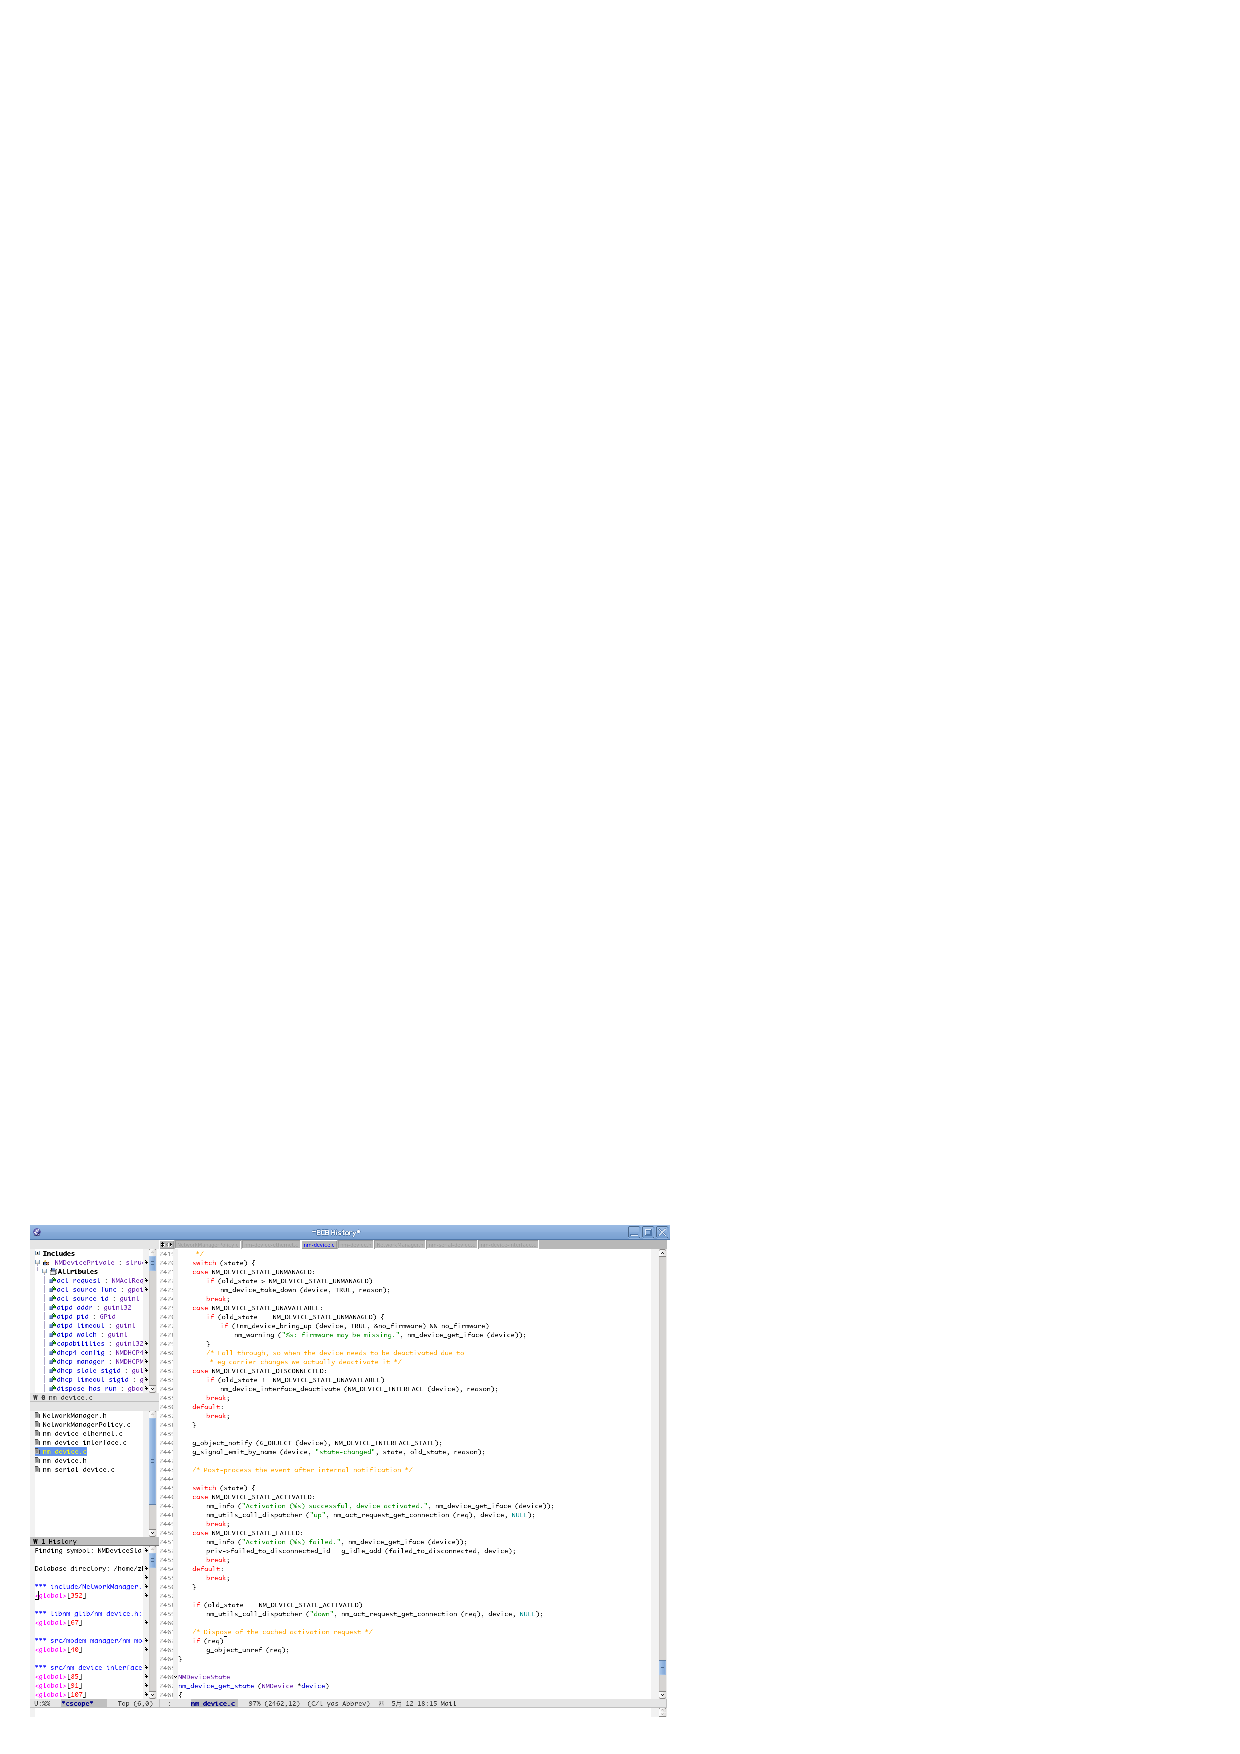
\includegraphics[width=15cm]{ecb-cscope.png}
\end{figure}

\subsection{cedect}
\subsubsection{基本cedect配置}
\subsubsection{其他}
\begin{itemize}
	\item M-x eassist-switch-h-cpp 快速切换h,cpp文件
	\item M-x eassist-list-methods 显示函数
\end{itemize}

\subsection{frame looks}
配置frame的默认属性,包括背景色,前景色,窗口位置大小,字体等等。
\begin{verbatim}
(setq default-frame-alist
      '((background-color . "black")
        (top . 20) (left . 40) (height . 40) (width . 128)
        (font . "monospace-11")
        (foreground-color . "#ffffff")))
\end{verbatim}


\subsection{只读模式}
\begin{verbatim}
C-x,C-q
\end{verbatim}
转为只读模式,在看代码的时候很有用
\subsection{emacs的一些启动项}
不带图形界面的启动
\begin{verbatim}
emacs -nw
\end{verbatim}
默认启动,不加载用户的配置文件
\begin{verbatim}
emacs -q 
\end{verbatim}
启动emacs的server模式,emacs在后台运行
\begin{verbatim}
emacs --daemon
\end{verbatim}
以后用emacsclient启动emacs前端,启动速度飞快,赶上vim
\input{../readme}
\end{document}
